\begin{figure}[t]
\begin{center}
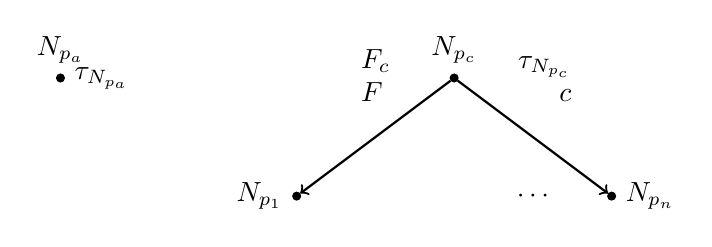
\begin{tikzpicture}[yscale=-1,
place/.style={circle,draw=black, fill=black, inner sep=0pt, 
              minimum size=1mm}]

 \node[place] (1st) at (1, 0) [label=above: $N_{p_{a}}$,
                               label=right: $\tau_{N_{p_{a}}}$] {};
	

\begin{scope}[xshift=4cm]
  \node[place] (1st) at (2, 0) [label=above: $N_{p_{c}}$,
                                label=right: 
       \begin{tabular}{l r}
         & $\tau_{N_{p_{c}}}$ \\
         & $c$\\
       \end{tabular},
       label=left:
       \begin{tabular}{l l}
         $F_c$ &\\
         $F$ &\\
       \end{tabular}] {};
  \node[place] (2nd) at (0, 1.5) [label=left: $N_{p_1}$] {};
  \node[place] (3rd) at (4, 1.5) [label=right: $N_{p_n}$]{}; 

  \node (dots) at (3,1.5) {$\cdots$};
	
  \draw[->, thick] (1st) -- (2nd);
  \draw[->, thick] (1st) -- (3rd);
\end{scope}

\end{tikzpicture}
\caption{Predicate Tree}
\label{Predicate Tree}
\end{center}   
\end{figure}
